\documentclass[landscape,a4paper]{extarticle}
\usepackage{caption}
\usepackage{multicol}
\usepackage[top=1em,bottom=1em,left=1em,right=1em]{geometry}
\usepackage[framemethod=tikz]{mdframed}
\usepackage{microtype}
\usepackage{pdfpages}
\usepackage{amsmath, amssymb, amsthm}
\usepackage{anyfontsize}
\usepackage[shortlabels]{enumitem}
\usepackage{graphicx, float}
\usepackage{ulem} % Using \uline{} instead of \underline{} will make the line closer to the word
\usepackage{xcolor}
\usepackage{tgschola}

\let\bar\overline

% Configure image directory
\graphicspath{{images/}}

\newenvironment{Figure}
  {\par\noindent\minipage{\linewidth}}
  {\endminipage\par\medskip}
  
% Remove caption labels
\captionsetup{labelformat=empty,labelsep=none}

% No paragraph indent
\setlength{\parindent}{0pt}

% No spaces between list items, no left margins
\setlist[enumerate]{nosep, leftmargin=*}
\setlist[itemize]{nosep, leftmargin=*}

% No spaces before and after math mode
\expandafter\def\expandafter\normalsize\expandafter{%
    \normalsize%
    \setlength\abovedisplayskip{0pt}%
    \setlength\belowdisplayskip{0pt}%
    \setlength\abovedisplayshortskip{-8pt}%
    \setlength\belowdisplayshortskip{2pt}%
}

\begin{document}
\fontsize{7}{8}\selectfont
\fontfamily{qcs}\selectfont
\begin{multicols*}{5}
	\textbf{\uline{Topic 0}}

	\textbf{CIA}
	\begin{enumerate}
		\item Confidentiality
		      \begin{itemize}
			      \item Prevention of unauthorized discolusre of information
		      \end{itemize}
		\item Integrity
		      \begin{itemize}
			      \item Prevention of unauthorized modification of information or processes
			      \item Non-repudiation
			      \item Authentication
		      \end{itemize}
		\item Availability
		      \begin{itemize}
			      \item Prevention of unauthorized withholding of information or resources
		      \end{itemize}
	\end{enumerate}
	\textbf{Threat model}

	\begin{itemize}
		\item The attacker's goals
		\item The attacker's capabilities
	\end{itemize}

	\textbf{Trade-off in security}
	\begin{itemize}
		\item Ease-of-use
		\item Performance
		\item Cost
	\end{itemize}

	\textbf{Threat-Vulnerability-Control}
	\begin{itemize}
		\item \textbf{Threat}: A set of circumstances that has the potential to cause harm (e.g. an
        attacker with control of the workstation in the LT could maliciously gather
        sensitive info like passwords)
        \item \textbf{Vulnerability}: A weakness in the system (e.g. anyone can reboot the
        workstation from USB or Disk to gain control)
        \item \textbf{Control}: A control, countermeasure, security mechanism is a mean to counter threats
        (e.g. restrict physical access to the workstation, disable USB booting)
        \item \textbf{A threat is blocked by control of a vulnerability}
	\end{itemize}
    
    \textbf{\uline{Topic 1: Encryption}}

    \textbf{1.1 Definition: Encryption/decryption/keys}

    \begin{Figure}
        \centering
        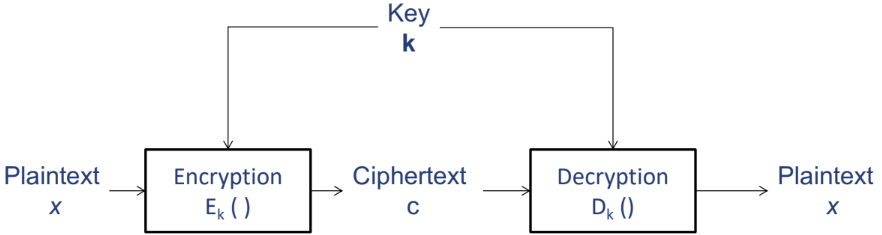
\includegraphics[width=\linewidth]{symmetric_key_encryption.png}
    \end{Figure}

    \begin{itemize}
        \item A symmetric-key encryption scheme consists of encryption and decryption
        \item A cipher must be correct and secure
        \begin{itemize}
            \item \textbf{Correctness}: For any plaintext $x$ and key $k$, $D_k(E_k(x)) = x$
            \item \textbf{Security}: Definition depends on the threat models. Informally,
            from the ciphertext, teh eavesdropper is unable to derive useful information of the
            key $k$ or the plaintext $x$, even if the eavesdropper can probe the system.
        \end{itemize}
        \item Probabilistic encryption: for the same $x$, there could be different $c$'s.
        But they all can be decrypted to the same $x$.
    \end{itemize}


    \textbf{1.2 Security Model and Requirement}
    
    \textbf{Threat model}
    \begin{itemize}
        \item Attacker's goal
        \begin{itemize}
            \item Total break (most difficult goal)
            \begin{itemize}
                \item Attacker wants to find the key
            \end{itemize}
            \item Partial break
            \begin{itemize}
                \item Attacker may want to decrypt a ciphertext but not interested in knowing the key
                \item Attacker may simply want to extract some info abt the plaintext (e.g. if it is a jpg or excel file)
            \end{itemize}
            \item Distinguishability (weakest goal)
            \begin{itemize}
                \item With some non-negligible probability of $>$ 1/2, the attacker acan correctly
                distinguish the ciphertexts of a given plaintext from the ciphertext of another given
                plaintext 
            \end{itemize}
        \end{itemize}
        \item Attacker's capability
        \begin{itemize}
            \item Ciphertext only attack
            \begin{itemize}
                \item Attacker is given a collection of ciphertext $c$. The attacker may 
                know some properties of the plaintext (e.g. the plaintext is an English sentence)
            \end{itemize}
            \item Known plaintext attack
            \begin{itemize}
                \item The attacker is given a collection of plaintext $m$ and their corresponding
                ciphertext $c$
                \item Attacker might get this as they know the header or part of the plaintext
            \end{itemize}
            \item Chosen plaintext attack (CPA)
            \begin{itemize}
                \item The attacker has access to an oracle. The attacker can choose and feed any plaintext
                $m$ to the oracle and obtain the corresponding ciphertext $c$ (all encrypted with
                the same key). The attacker can access the oracle many times, as long as within the attacker's
                compute power. He can see the ciphertext and then choose the next input. This black-box is an
                \textbf{encryption oracle}. 
                \item e.g. attacker has access to a smartcard
                \item e.g. attacker can eavesdrop
            \end{itemize}
            \item Chosen ciphertext attack (CCA2)
            \begin{itemize}
                \item Same as CPA but the attacker chooses the ciphertext and the black-box
                outputs the plaintext. The black-box is a \textbf{decryption oracle}.
                \item Padding oracle is a weaker form of a decryption oracle.
            \end{itemize}
        \end{itemize}
    \end{itemize}

    From defender's POV, want a cipher that can protect against the attacker with the highest
    capability. Cipher is secure against CCA2 (decryption oracle) $\implies$ secure
    against CPA (encryption oracle)

    \textbf{1.3 Classical ciphers + illustration of attacks}

    \textbf{1.3.1 Substitution cipher}

    \begin{itemize}
        \item Plaintext and ciphertext are both strings over a set of symbols $U$.
        \item The key is a 1-1 onto func from $U$ to $U$
        \item Key space: set of all possible keys
        \item Key space size: total number of possible keys
        \item Key size/length: number of bits required to represent a key
        \item Attacks
        \begin{enumerate}
            \item Exhaustive search (examine all possible keys 1 by 1)
            \begin{itemize}
                \item Running time depends on size of key space
                \item If the table size is 27, the key can be represented by a sequence of 27
                symbols. The size of key space is 27!. Exhaustive search eneds to carry out 27!
                loops, which is infeasible using current compute power.
            \end{itemize}
            \item Known plaintext attack
            \begin{itemize}
                \item Given sufficiently long ciphertext, the full table can be found
                \item Substitution cipher is not secure under known plaintext attack.
            \end{itemize}
            \item Ciphertext only attack
            \begin{itemize}
                \item Given that the attacker knows that the plaintext is an English sentence,
                he can do frequency analysis attack. The frequency of letters used in English is 
                not uniform. Given a sufficiently long ciphertext, attacker may correctly guess the plaintext by 
                mapping frequent characters in the ciphertext to the frequent character in English.
            \end{itemize}
        \end{enumerate}
    \end{itemize}

    \textbf{1.3.2 Permutation cipher}
    \begin{Figure}
        \centering
        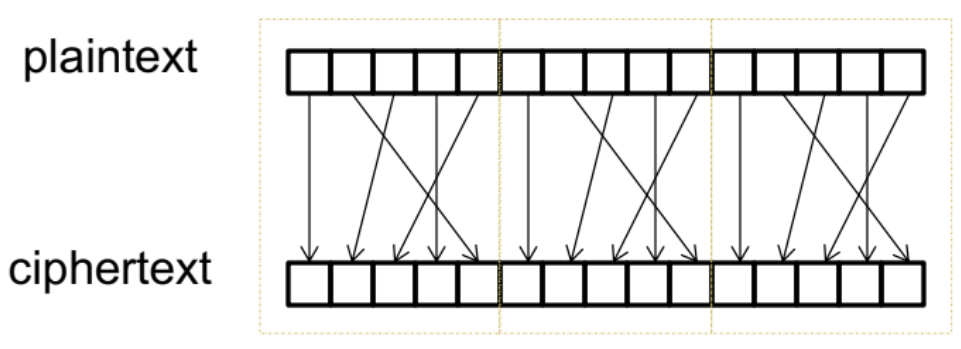
\includegraphics[width=\linewidth]{permutation_cipher.png}        
    \end{Figure}
    \begin{itemize}
        \item AKA transposition cipher
        \item First group the plaintext into blocks of $t$ characters, then apply a secret
        permutation to each block by shuffling the characters
        \item The key is the secret permutation, which is a 1-1 onto func $e$ from $\{1, 2, \ldots, t\}$
        to $\{1, 2, \ldots, t\}$. $t$ can also be part of the key.
        \item Attack
        \begin{itemize}
            \item Fails under known-plaintext attack
            \item Easily broken under ciphertext only attack if the plaintext is English text
        \end{itemize}
    \end{itemize}

    \textbf{1.3.3 One Time Pad}

    \textbf{Properties of xor}: 
    \begin{itemize}
        \item Commutative: $A \oplus B = B \oplus A$
        \item Associative: $A \oplus (B \oplus C) = (A \oplus B) \oplus C$
        \item Identity element: $A \oplus 0 = A$
        \item Self-inverse: $A \oplus A = 0$
    \end{itemize}

    \textbf{One Time Pad}
    \begin{itemize}
        \item Encryption: plaintext xor key bit by bit
        \item Decryption: ciphertext xor key bit by bit
        \item Key is only used once, so 1GB of plaintext would need a 1GB key to encrypt
        \item Security
        \begin{itemize}
            \item From a pair of ciphertext and plaintext, attacker can derive the key
            but useless bc key won't be used anymore
        \end{itemize}
    \end{itemize}

    \textbf{1.4 Modern ciphers + recommended key length}

    \textbf{1.4.2 Block cipher \& mode of operations}

    DES/AES are known as block ciphers. Block ciphers have a fixed size of input/output.
    AES: 128 bits (16 bytes). 

    Large plaintext is divided into blocks before applying the block cipher.

    \textbf{ECB (electronic code book) mode}
    \begin{Figure}
        \centering
        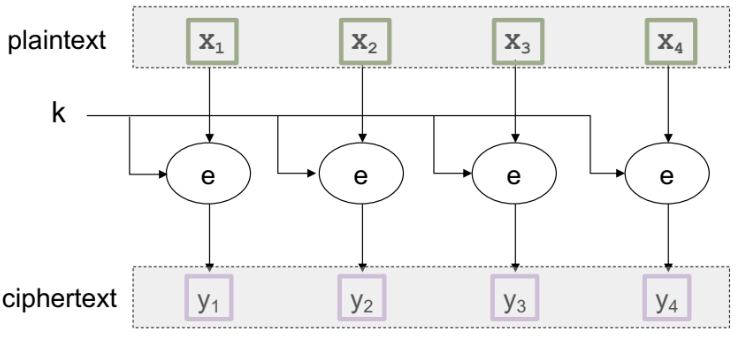
\includegraphics[width=\linewidth]{ecb_encryption.png}        
    \end{Figure}
    \begin{Figure}
        \centering
        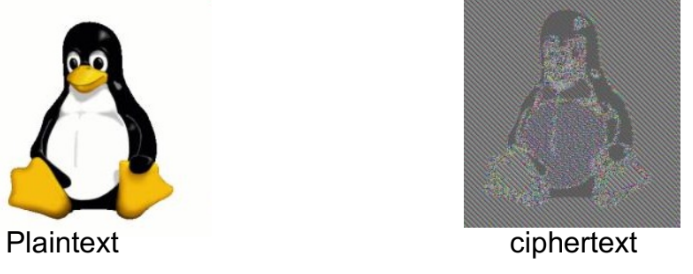
\includegraphics[width=\linewidth]{ecb_penguin.png}        
    \end{Figure}

    \textbf{CBC (cipher block chaining) mode on AES}
    \begin{itemize}
        \item Initialization vector (IV) is an arbitrary value chosen during encryption, 
        must be different in different encryptions. 
        \item In CBC mode, IV must be unpredictable, else it is susceptable to BEAST attack.
        \item If IV is randomly chosen, it is unpredictable
    \end{itemize}
    \begin{Figure}
        \centering
        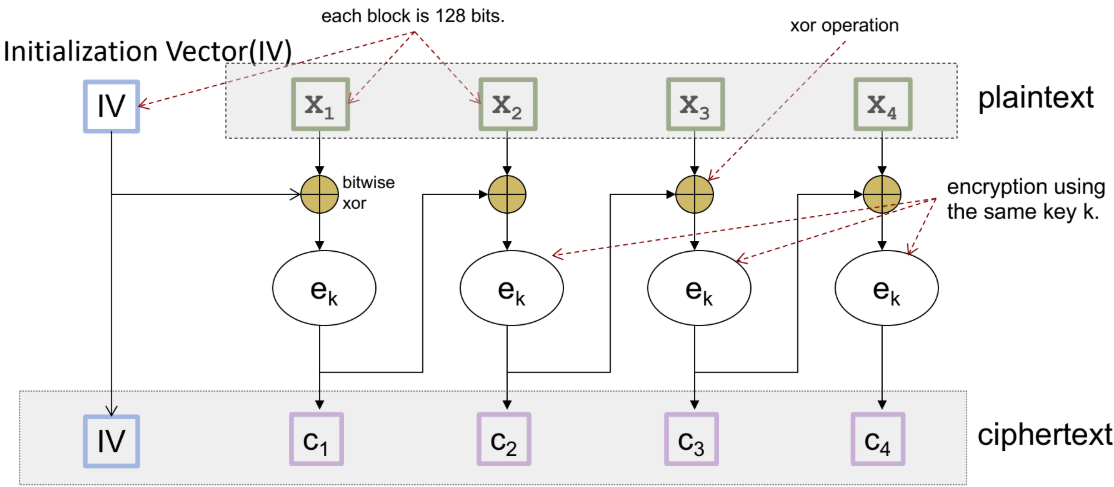
\includegraphics[width=\linewidth]{cbc_encryption.png}        
    \end{Figure}
    \begin{Figure}
        \centering
        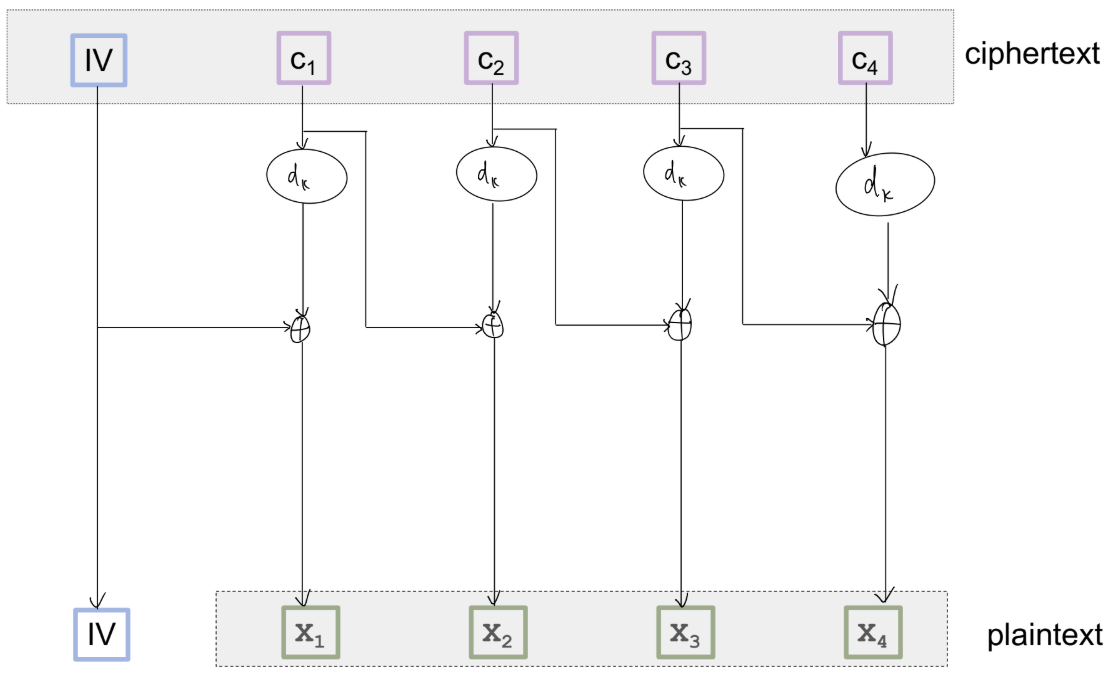
\includegraphics[width=\linewidth]{cbc_decryption.png}        
    \end{Figure}

    \textbf{CTR (counter) mode}
    \begin{Figure}
        \centering
        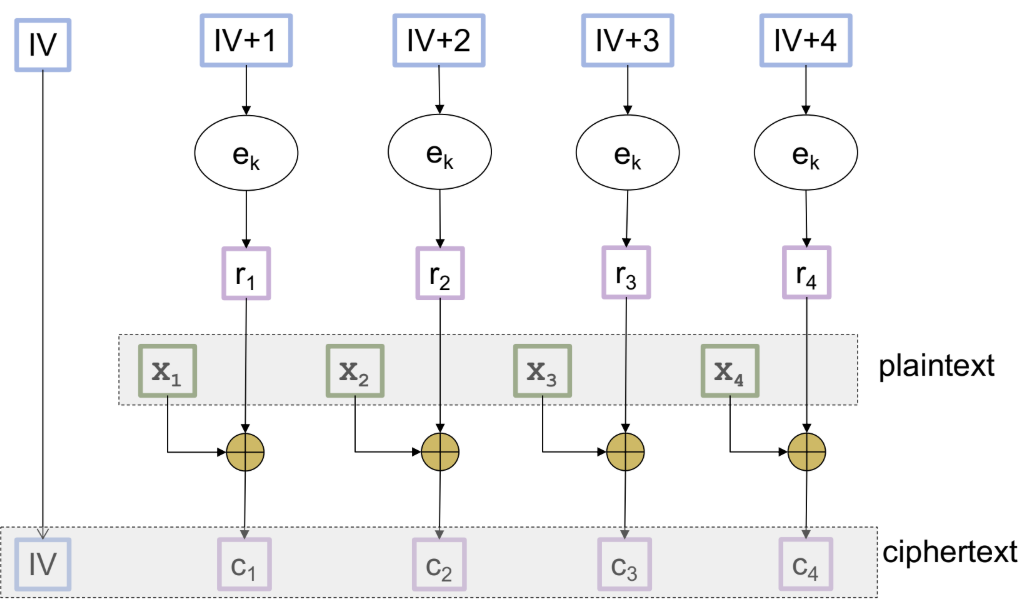
\includegraphics[width=\linewidth]{ctr_encryption.png}        
    \end{Figure}
    \begin{Figure}
        \centering
        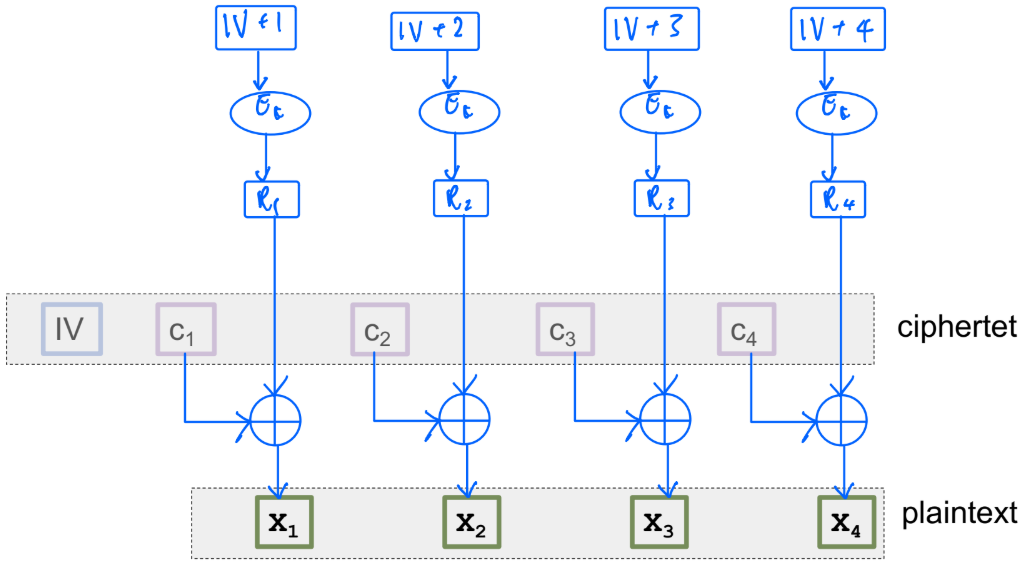
\includegraphics[width=\linewidth]{ctr_decryption.png}        
    \end{Figure}

    \textbf{GCM mode (Galois/counter)}

    Authenticated encryption, ciphertext consists of extra tag for authentication.
    Secure in the presence of decryption oracle.

    \textbf{1.4.3 Stream cipher and IVs}

    Stream cipher is bit by bit. CTR mode is a "stream cipher" but it is not bit by bit.
    \begin{Figure}
        \centering
        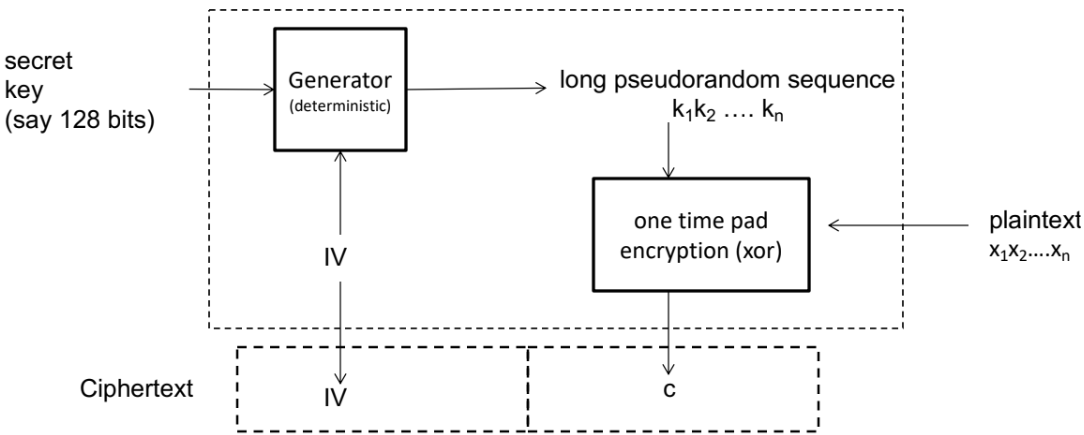
\includegraphics[width=\linewidth]{stream_cipher.png}        
    \end{Figure}

    \begin{itemize}
        \item Need IV and no two IVs can be the same
    \end{itemize}

    \textbf{Stream cipher without IV}
    \begin{Figure}
        \centering
        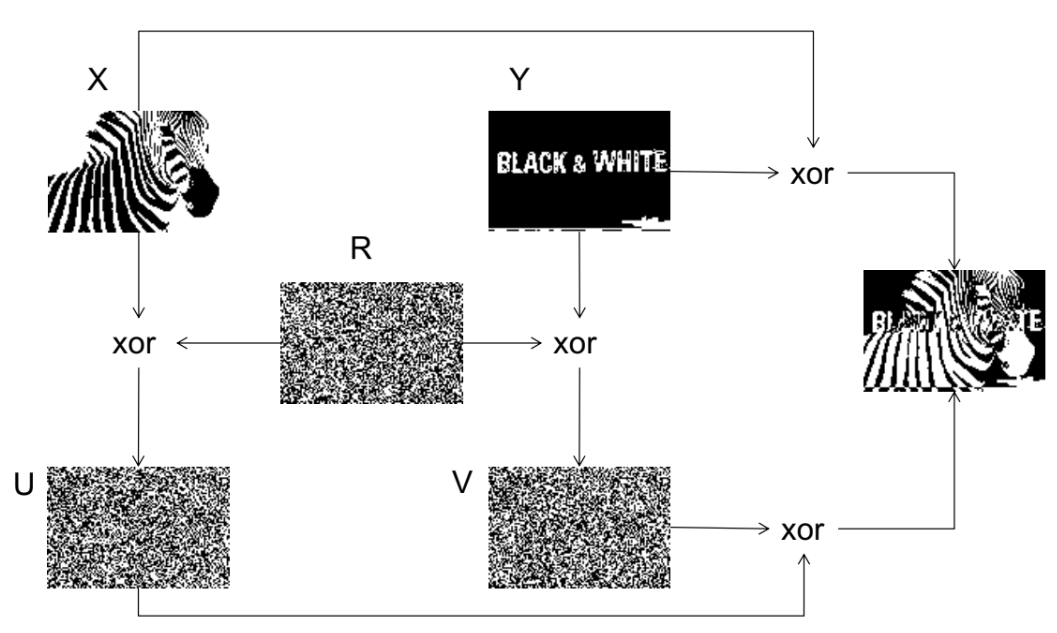
\includegraphics[width=\linewidth]{stream_cipher_without_iv.png}        
    \end{Figure}

    \textbf{Stream cipher with IV}
    \begin{Figure}
        \centering
        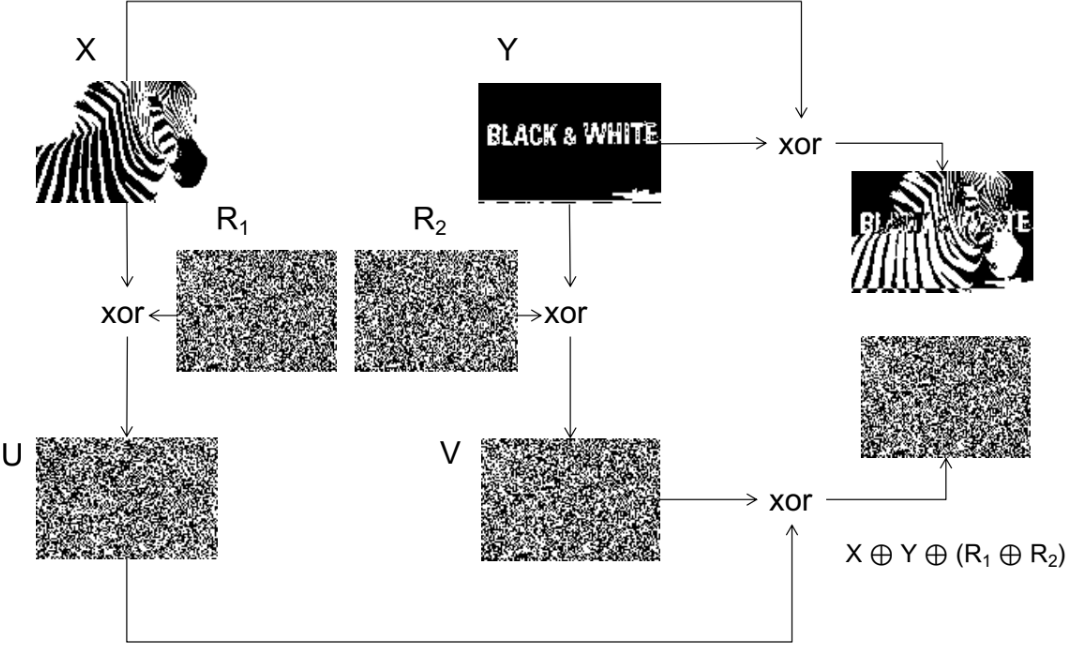
\includegraphics[width=\linewidth]{stream_cipher_with_iv.png}        
    \end{Figure}

    \begin{itemize}
        \item IV makes an encryption probabilistic
    \end{itemize}
    
    \textbf{1.5 Examples of attacks on crypto}

    \textbf{1.5.1 Meet-in-the-middle}

    \begin{itemize}
        \item DES is not secure $\rightarrow$ improve by encrypting multiple times using different
        keys
        \item Consider double encryption under known plaintext attack. Attacker has $m$ and $c$ and
        wants to know $k_1$, $k_2$.
        \item Using exhaustive search, amount of DES encryption/decryption would be $2^{56+56}$
        \item Hence use meet-in-the-middle attack.
        % Compute sets $C$ and $M$, where $C$ contains
        % ciphertexts of $m$ encrypted with all possible keys and $M$ contains plaintexts of $c$ decrypted
        % with all possible keys. Then find all common elements (likely only 1) in $C$ and $M$. From 
        % common elements, obtain the 2 keys.
        \item for $k$-bit keys, this reduces the number of crypto operations to $2^{k + 1}$
    \end{itemize}

    \begin{Figure}
        \centering
        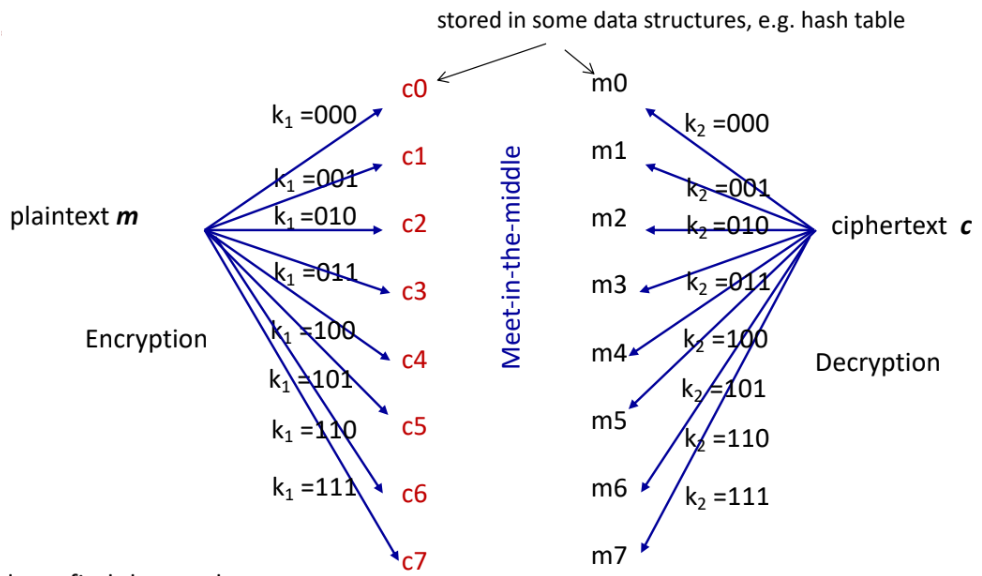
\includegraphics[width=\linewidth]{meet_in_the_middle.png}        
    \end{Figure}

    \textbf{Tradeoff with time and space}

    \begin{Figure}
        \centering
        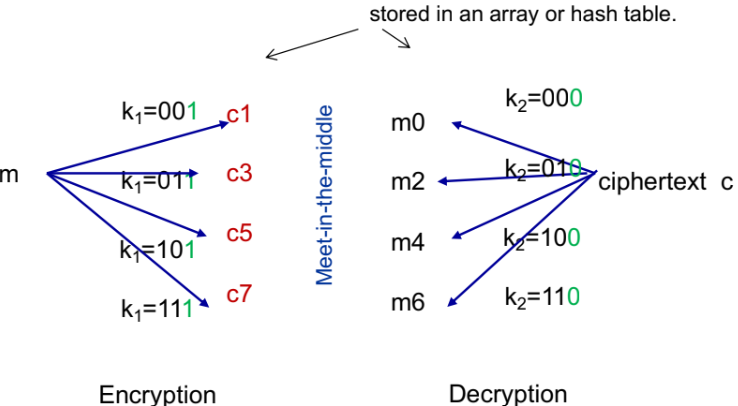
\includegraphics[width=\linewidth]{meet_in_the_middle_tradeoff.png}        
    \end{Figure}

    \begin{itemize}
        \item Last bit of $k_1$ fixed to 1, last bit of $k_2$ fixed to 0
        \item Perform meet-in-the-middle on the first 2 bits of $k_1$ and $k_2$
    \end{itemize}

    \textbf{1.5.2 Padding Oracle}

    Plaintext needs to be padded to split into blocks

    \begin{itemize}
        \item PKCS\#7 is a padding standard
    \end{itemize}

    \begin{Figure}
        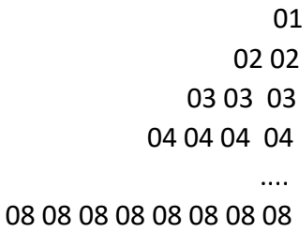
\includegraphics[width=0.5\linewidth]{pkcs7.png}        
    \end{Figure}

    \textbf{Padding oracle attack}

    Attack model: 

    Attacker has:
    \begin{enumerate}
        \item Ciphertext (iv, c) where the ciphertext was encrypted using $k$
        \item Access to a padding oracle
    \end{enumerate}
    Attacker's goal: plaintext of (iv, c)

    Padding oracle input is ciphertext, output is YES if the plaintext is in the correct
    padding format else NO

    \textbf{Padding oracle attack on AES CBC mode}

    Attacker knows:

    \begin{Figure}
        \centering
        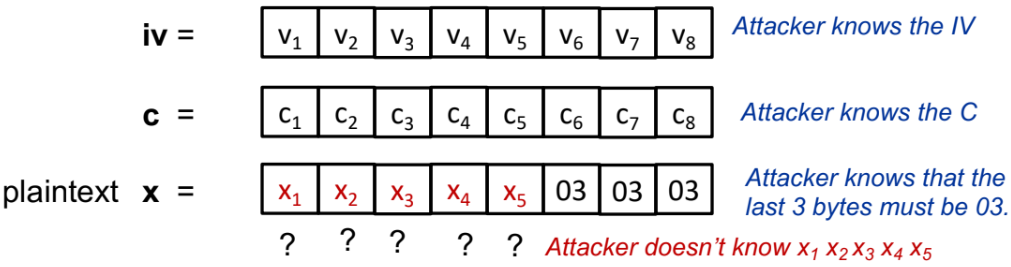
\includegraphics[width=\linewidth]{padding_oracle_attacker_knowledge.png}
    \end{Figure}

    \begin{Figure}
        \centering
        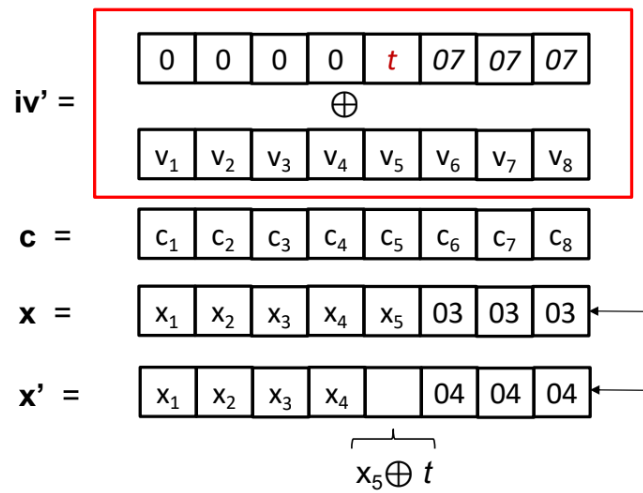
\includegraphics[width=\linewidth]{padding_oracle_attack.png}
    \end{Figure}

    \begin{align*}
        iv \oplus d(c) &= 03\\
        iv' \oplus d(c) &= 04
    \end{align*}

    xor the 2 tgt to get $iv' = 07 \oplus iv$

    \begin{align*}
        iv' &= iv \oplus 00\ 00 \ldots t\ 07\ 07\ 07\\
        d(C_5) \oplus t \oplus V_5 &= 04\\
        d(C_5) \oplus V_5 \oplus t &= 04\\
        d(C_5) \oplus V_5 &= x_5\\
        x_5 \oplus t &= 04\\
        x_5 &= 04 \oplus t
    \end{align*}
    
    Keep guessing $t$ until padding oracle outputs YES, then we know $x_5$

    To get next byte:
    \begin{Figure}
        \centering
        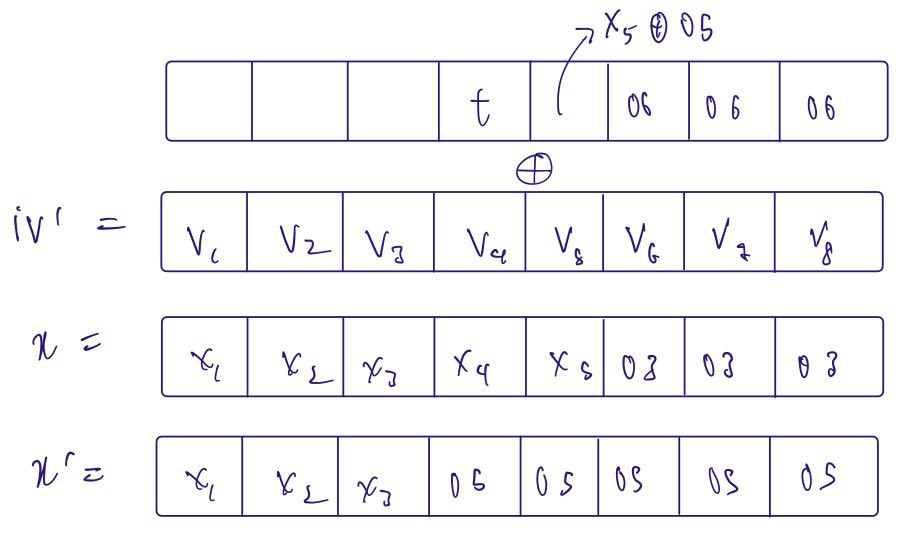
\includegraphics[width=\linewidth]{padding_oracle_next_byte.jpg}
    \end{Figure} 

    \textbf{1.6 Pitfalls in usages and implementations}
    \begin{enumerate}
        \item Wrong choice of IV / reusing one-time pad
        \item Randomness is predictable
        \item Modify existing or design your own encryption scheme
        \item Reliance on obscurity: Kerkchoff's principle
        \begin{itemize}
            \item Kerkchoff's principle: A system should be secure ven if everything about the
            system, except the secret key, is public knowledge
        \end{itemize}
    \end{enumerate}

    \textbf{\uline{Topic 2: Authentication Credential}}

    \textbf{Authentication}

    Authentication is the process of assuring that the communicating identity, or origin of a
    piece of information, is the one that it claims to be.

    \begin{itemize}
        \item Authentication implies integrity.
    \end{itemize}

    \textbf{Data-origin authentication}: is a piece of data generated by an authentic entity?
    \begin{itemize}
        \item Signature or MAC (message authentication code)
    \end{itemize}

    \textbf{Commnication authentication}: is the enitity interacting with the verifier an authentic entity?
    \begin{itemize}
        \item Authentication protocol
    \end{itemize}

    \textbf{2.2 Password}

    \textbf{Password vs key}

    Passwords are generated by human and can be remembered by human. Keys are binary sequences that are infeasible to be 
    remembered by humans.

    \textbf{Entropy:} The amount of uncertainty that an attacker faces to determine the value of a secret. 
    Stated in bits. a value with $n$ bits of entropy has the same degree of uncertainty as a uniformly distributed $n$-bit
    random value.

    \textbf{Password system}

    \begin{enumerate}
        \item Bootstrapping
        \begin{itemize}
            \item User and server establish a common password, server keeps a password file keeping the 
            identity and the corresponding password
            \item Password established during boostrapping either by a default password
            or by the server/user choosing a password and sending it to the user/server through another
            communication channel
        \end{itemize}
        \item Authentication
        \begin{itemize}
            \item Server authenticates an entity. An entity who can convince the server that it knows
            the password is deemed to be authentic.
        \end{itemize}
        \item Password reset
        \begin{itemize}
            \item Need to authenticate the entity before allowing the entity to change password.
            \item Need another credential (other than the old password) to authenticate bc ppl might 
            want to reset password when they forget
            \item Can be done through OTP, security question (not secure as entropy of answers is 
            lower than the password)
        \end{itemize}
    \end{enumerate}

    \textbf{Attack on passwords}

    \textbf{2.2.1 Attack on Bootstrapping}
    \begin{itemize}
        \item Attacker intercepts the password during bootstrapping, e.g. if password
        is sent through postal mail, an attacker steals the mail to get the password
        \item Attacker uses the "default" passwords
        \begin{itemize}
            \item Mitigation: require the user to change password after first login
        \end{itemize}
        \item Example: zoom flaw allowed account hijacking
    \end{itemize}

    \textbf{2.2.2 Attack on Password Reset}
    \begin{itemize}
        \item Mechanism of security questions weakens the password system, but it is less
        common now
        \item Social engineering + password reset
    \end{itemize}

    \begin{Figure}
        \centering
        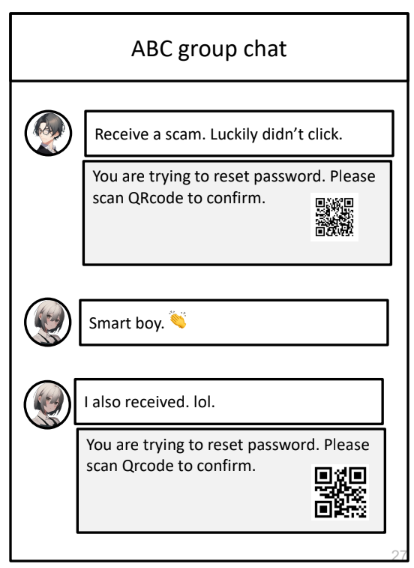
\includegraphics[width=0.9\linewidth]{social_engineering_pw_reset.png}
    \end{Figure}

    \textbf{2.2.3 Searching for the password}

    \textbf{Dictionary attacks}
    \begin{itemize}
        \item Test passwords using a dictionary that could contain words from English dict, known
        compromised passwords, etc.
        \item Also test combinations of words in the dictionary. e.g. combinations of 2 words, all possible capitalizations
        of letters in each word, substituting `a' with `@', etc.
        \item \textbf{Online dictionary attack}
        \begin{itemize}
            \item To test a password, attacker must itneract with the authentication system
        \end{itemize}
        \item \textbf{Offline dictionary attack}
        \begin{itemize}
            \item Attacker first obtains some information $D$ about the password, possibly by sniffing the login session
            of an authentic user, or by interacting with the server. (e.g. attacker obtains the hashed password)
            \item Next, the user carries out dictionary attack using $D$ without interacting with the system (e.g. attacker
            compares the hashed password with the hashed words in dictionary)
        \end{itemize}
        \item Guessing password from social information: attacker gathers social information
        about the user, e.g. phone no., and infers the password by constructing a dictionary
        using words extracted from the social media
    \end{itemize}

    \textbf{2.2.4 Stealing the password}
    \begin{enumerate}
        \item Sniffing
        \begin{itemize}
            \item Shoulder surfing: look-over-the-shoulder attack
            \item Sniffing the communication: Some systems simply send the password over
            the public network in clear (i.e. not encrypted), e.g. FTP, Telnet, HTTP
            \item Sniff wireless keyboards that employ insecure encryption method
            \item Using sound made by keyboard
            \item Viruses, key-logger
            \begin{itemize}
                \item Key-logger captures keystrokes and sends the info back to the attacker.
                \item Can be in the form of software (viruses) or hardware.
            \end{itemize}
        \end{itemize}
        \item Phishing
        \begin{itemize}
            \item Victim is tricked into voluntarily sending the password to the attacker
            \item Asks for password under false pretense
        \end{itemize}
        \item Spear Phishing
        \begin{itemize}
            \item Phishing that is targeted to a particular small group of users, e.g. NUS staff
        \end{itemize}
    \end{enumerate}

    \textbf{Phishing Prevention}
    \begin{itemize}
        \item User training
        \item Blacklisting, e.g. phishtank.com
        \item Visually spot by ensuring that there is a padlock in the address bar and that the 
        domain name in the url is correct
    \end{itemize}

    \textbf{2.2.5 Password strength}
    \begin{itemize}
        \item We quantify the key-strength by the size of the key if best-known attack is exhaustive search.
        \item If best-known attack is faster, then we quanitfy it by its equivalent in exhaustive search.
    \end{itemize}

    \textbf{Using strong password}
    \begin{itemize}
        \item Truly random password: password is chosen randomly among all possible keys using an automated passsword
        generator. High entropy but difficult to remember.
        \item User selection: 
        \begin{itemize}
            \item Mnemonic method
            \item Altered passphrases
            \item Combining and altering word
        \end{itemize}
        \item Usability:
        \begin{itemize}
            \item Strong passwords are difficult to remember
            \item It is difficult to enter alphanumeric passwords into mobile devices. There are alternatives,
            e.g. graphical or gesture-based
        \end{itemize}
    \end{itemize}

    \textbf{Password entropy}

    Suppose a set $P$ contains $N$ unique passwords. A password is chosen by randomly picking
    a password from $P$.     
    \begin{equation*}
        -\sum_{i=1}^N p_i \log_2p_i
    \end{equation*}
    where $p_i$ is the probability that the $i$-th password is picked.

    If the password is chosen uniformly, each password in $P$ has probability of $1/N$ of
    being chosen. The entropy of the password is
    \begin{equation*}
        log_2N \text{ bits}
    \end{equation*}

    For the entropy to be highest for a set of $N$ items, $p_i$ must be $1/N$

    \textbf{Additional protection to password files}

    Password file should be hashed and salted
    \begin{Figure}
        \centering
        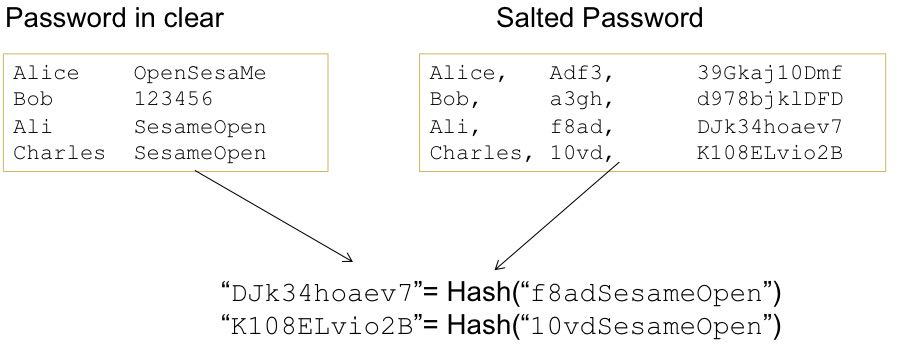
\includegraphics[width=\linewidth]{hashed_salted.jpg}        
    \end{Figure}

    Make it harder for rainbow table attack

    \textbf{2.3 Biometric}
    Biometric data is the password

    \begin{align*}
        &\text{FMR (false positive)}\\
       =\ &\frac{\text{no. of successful false matches (B)}}{\text{no. of attempted false matches (B + D)}}
    \end{align*}
    \vspace{1px}
    \begin{align*}
        &\text{FNMR (false negative)}\\
       =\ &\frac{\text{no. of rejected genuine matches (C)}}{\text{no. of attempted genuine matches (A + C)}}
    \end{align*}
    \begin{Figure}
        \centering
        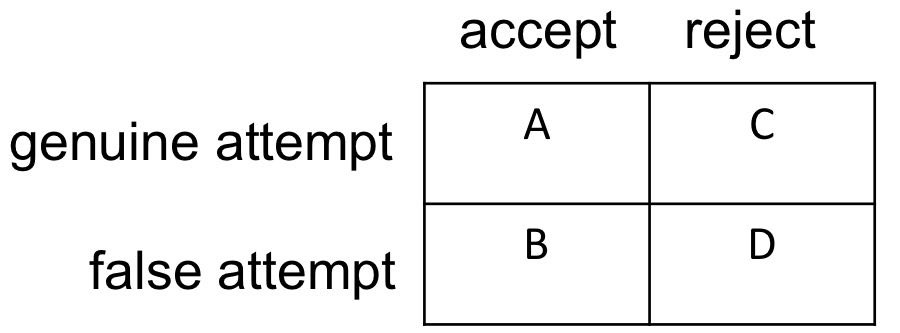
\includegraphics[width=0.8\linewidth]{fmr_fnmr.jpg}        
    \end{Figure}
    Threshold: FNMR/FMR. Lower threshold more relax, higher threshold more stringent

    \textbf{Attack on biometric system}

    Biometric data can be spoofed, use liveness detection e.g. temperature sensor in fingerprint scanner

    \textbf{2.4 n-factor Authentication and Multi-Step Verification}

    \textbf{n-factor Authentication}

    Requires at least 2 different authentication ``factors''

    \begin{enumerate}
        \item Something you know: password, PIN
        \item Something you have: Security token, smart card, phone, ATM card
        \item Who you are: Biometric
    \end{enumerate}

    \textbf{Multi-Step Verification}

    If both are the same category of factors (2 passwords, both are something you know) 
    then it is 2-step verification

    \textbf{\uline{Topic 3: Authenticity (data origin)}}

    \textbf{3.1 PKC}

    \begin{itemize}
        \item With multiple identitites, many pairs of symmetric keys are required.
        \item Symmetric key requires both entities to know each other before the actual
        communication session. Hence use public key encryption.
    \end{itemize}

    \begin{Figure}
        \centering
        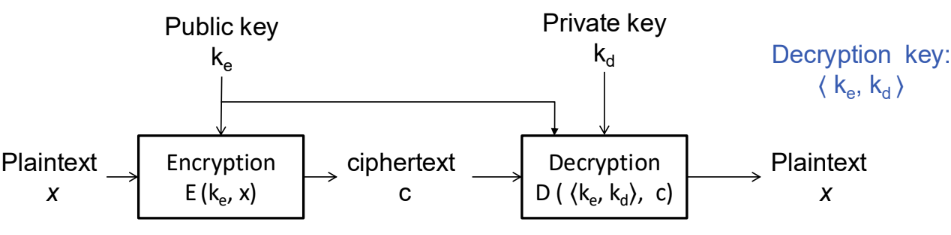
\includegraphics[width=\linewidth]{public_key_encryption.png}
    \end{Figure}

    \textbf{Popular PKC schemes}
    \begin{itemize}
        \item RSA
        \item ElGamal
        \item Paillier
        \item Post-quantum cryptography
    \end{itemize}

    \textbf{3.1.1 RSA}

    \begin{enumerate}
        \item Owner randomly chooses 2 large primes $p, q$ and computes $n=pq$
        \item Owner randomly chooses an encryption exponent $e$ s.t. $\gcd(e, (p - 1)(q - 1)) = 1$
        \item Owner finds decryption exponent $d$ where $d e \mod(p - 1)(q - 1) = 1$
        \item Owner publishes $\langle n, e \rangle$ as public key, and safe-keeps $d$ as the private key
    \end{enumerate}

    \begin{Figure}
        \centering
        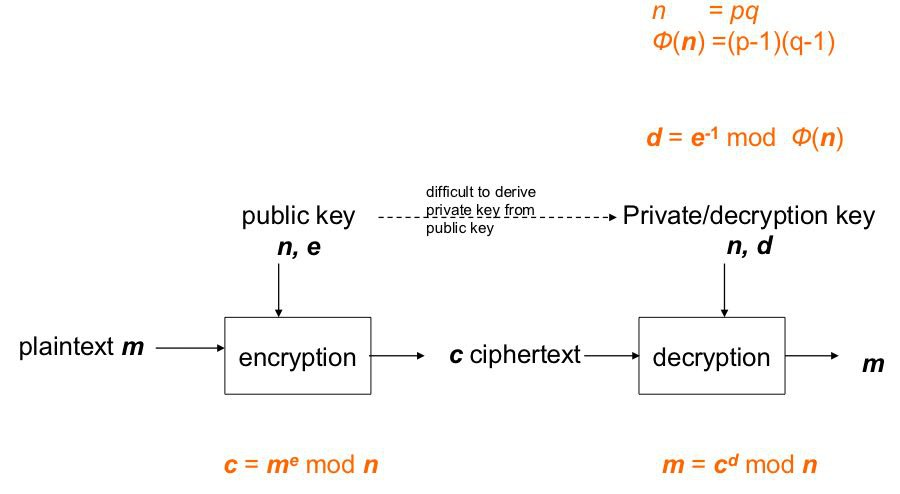
\includegraphics[width=\linewidth]{textbook_rsa.jpg}        
    \end{Figure}

    Got algo to find $d$ given $e, p, q$. For faster speed, choose small $e$. Common value is 65537.
    $e$ is not a secret in such cases

    \textbf{3.1.2 Security of RSA}

    Getting RSA private key from public key is as difficult as factorizing $n$.

    \textbf{Padding of RSA}

    \begin{itemize}
        \item Some forms of IV is required so that encryption of the same plaintext at different
        times would give different ciphertexts. Additional padding required for security.
    \end{itemize}

    \textbf{3.1.3 Efficiency}

    RSA encryption/decryption is significantly slower than AES. To encrypt a large file, it would 
    be very slow to directly apply RSA (or other PKC).

    Can use PKC to encrypt a symmetric key then use AES for encryption

    \textbf{3.2 Data Authenticity}

    \textbf{Security requirement of hash}

    \begin{itemize}
        \item Collision-resistant
        \begin{itemize}
            \item Collision: Find 2 different messages $m_1, m_2$ s.t. $h(m_1) = h(m_2)$
        \end{itemize}
        \item 2nd pre-image resistant
        \begin{itemize}
            \item 2nd pre-image: Given $m_1$, find $m_2$ s.t. $h(m_1) = h(m_2)$
        \end{itemize}
        \item One-way
        \begin{itemize}
            \item Pre-image: Given $y$, find $m$ s.t. $h(m) = y$
        \end{itemize}
    \end{itemize}

    \textbf{Application of unkeyed hash}

    When downloading something from a website, match the hash of the file with the checksum
    displayed in the browser.

    \begin{Figure}
        \centering
        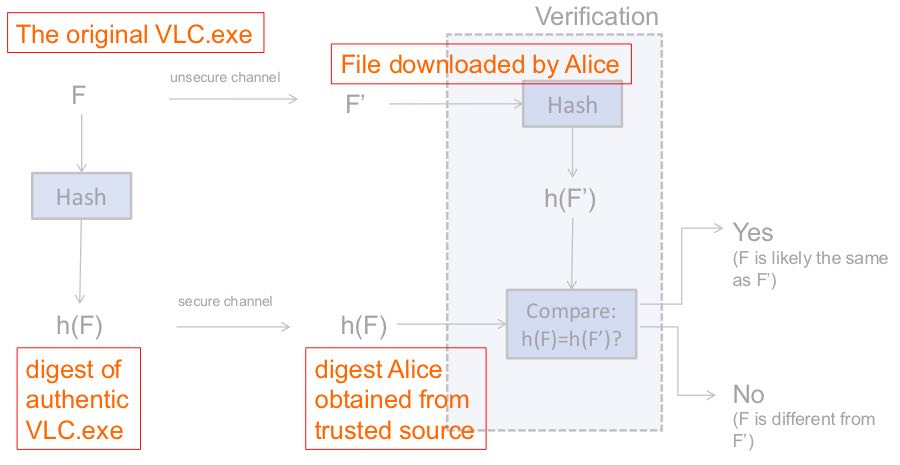
\includegraphics[width=\linewidth]{hash_application_vlc.jpg}
    \end{Figure}

    If not 2nd pre-image resistant, can be attacked

    \textbf{3.3 Data Origin Authenticity (mac), keyed}

    Keyed-hash is a function whose input is an arbitrary large message and a secret key, output is a
    fixed-size mac (message authentication code)
    \begin{itemize}
        \item Security requirement (forgery): Even if attacker sees multiple valid pairs of messages and their
        corresponding mac, it is difficult for the attacker to forge the mac of a message not seen before
        \item CBC-MAC: based on AES operated under CBC mode
        \item HMAC: Hashed-based MAC based on SHA
    \end{itemize}

    \textbf{Application of mac}

    Same situation as before but dh secure channel to deliver digest. Protect the digest
    with the help of some secrets.
    \begin{itemize}
        \item In symmetric key setting, called mac
        \item In public key setting, called digital signature
        \item mac typically appended to file, also called authentication tag or authentication code
    \end{itemize}

    \textbf{3.4 Data Origin Authenticity (Signature)}

    Public key version of MAC is called signature
    \begin{itemize}
        \item Owner uses private key to generate signature, public uses public key to verify
        signature
    \end{itemize}

    \begin{Figure}
        \centering
        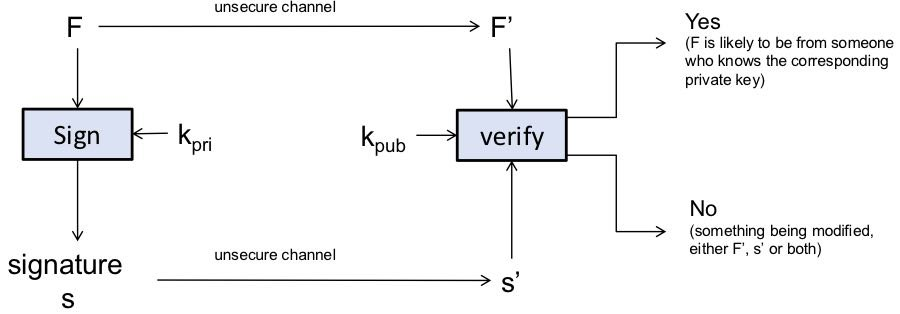
\includegraphics[width=\linewidth]{signature.jpg}
    \end{Figure}
    Signature is appended to the file F
    \begin{itemize}
        \item Signature scheme achieves \textbf{non-repudiation}
    \end{itemize}
    \begin{Figure}
        \centering
        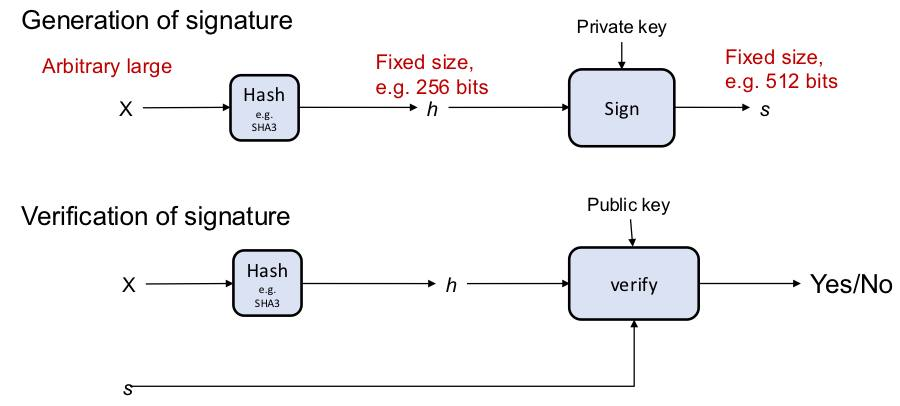
\includegraphics[width=\linewidth]{signature_generation_verification.jpg}
    \end{Figure}
    hash and sign / hash and encrypt

    \textbf{3.5.1 Birthday Attacks}

    Birthday attack is used to find collision. 

    Suppose we have $M$ messages, and each message is tagged with a value randomly chosen from $\{1,2,3, \ldots, T\}$.
    THen the probability that there is a pair of messages tagged with the same value is approx

    \begin{equation*}
        1-e^{\left(-\frac{M^2}{2T}\right)}
    \end{equation*}

\end{multicols*}
\end{document}